%% IJCAI-format METHOD paper, draft v0.4 (2026-10-19).
%% Changes from v0.3 (main.tex / main_v0.3.tex): offline probe audit on frozen models (policy, trajectory and reward
%% probes; Section 8, Table 3); E1 reported together with a same-seed repeat; E1-F described as interrupted; the main
%% experiment moved to a six-agent, goal-separated, team-reward task (results pending); Random-gated implemented
%% (not yet trained); reward-correlation baseline added; claims lowered to single-seed level; prose rewritten.
%% \pilot = single training seed; \tbd = to be filled when runs finish. Earlier drafts: main_v0.1.tex .. main_v0.3.tex.
%% Upload the official IJCAI author-kit files (ijcai27.sty or ijcai26.sty, named.bst) next to this file.
\IfFileExists{ijcai27.sty}{\def\ijcaistyle{ijcai27}}{\IfFileExists{ijcai26.sty}{\def\ijcaistyle{ijcai26}}{}}
\ifdefined\ijcaistyle
  \documentclass{article}
\else
  \documentclass[twocolumn,10pt]{article}
\fi
\pdfpagewidth=8.5in
\pdfpageheight=11in
\ifdefined\ijcaistyle
  \usepackage{\ijcaistyle}
\else
  \usepackage[letterpaper,margin=0.75in,columnsep=0.25in]{geometry}
  \usepackage[round]{natbib}
\fi
\usepackage{times}
\usepackage{soul}
\usepackage{url}
\usepackage[utf8]{inputenc}
\usepackage[small]{caption}
\usepackage{graphicx}
\usepackage{amsmath}
\usepackage{amssymb}
\usepackage{amsthm}
\usepackage{booktabs}
\usepackage{xcolor}
\usepackage{algorithm}
\usepackage{algpseudocode}
\urlstyle{same}

\newtheorem{proposition}{Proposition}
\newtheorem{lemma}{Lemma}
\newtheorem{assumption}{Assumption}
\newtheorem{definition}{Definition}
\theoremstyle{remark}
\newtheorem{remark}{Remark}

\newcommand{\todo}[1]{\textcolor{red}{[TODO: #1]}}
\newcommand{\tbd}{\textcolor{red}{TBD}}
\newcommand{\pilot}{\textsuperscript{\textcolor{gray}{$\dagger$}}}
\newcommand{\sg}{\operatorname{sg}}
\newcommand{\JS}{\operatorname{JS}}
\newcommand{\KL}{\operatorname{KL}}
\newcommand{\ours}{PGCT}

\title{Probe-Gated Critic Transfer:\\ Local Teammate Inference for Selective Critic Sharing\\ in Multi-Agent Reinforcement Learning}
\author{Anonymous submission}

\begin{document}
\maketitle

\begin{abstract}
Agents that share an environment may belong to teams with different objectives without knowing who their teammates
are. In Probe-Gated Critic Transfer (\ours{}), neighbouring agents compare their action distributions on a fixed bank of
probe observations, treat a neighbour as a teammate when the smoothed Jensen--Shannon divergence falls below a threshold,
and distil that neighbour's critic on probe inputs. We state when this gate recovers the local team relation (a
separation margin larger than twice the tracking error, which we bound by the policy change between measurements), bound
the bias that a wrong donor introduces, and show that teams whose induced decision problems coincide cannot be told apart
by comparing responses to identical inputs. The evidence so far is limited. On a four-agent warehouse task with symmetric
team goals, one training seed gave \ours{} a higher mean throughput than independent PPO (11.7 vs.\ 10.4 deliveries per
episode up to 6.4M steps), but the gate linked agents of different teams, and a repeat of the same seed shifted the
learning onset of the transfer variants by 0.3--2.2M steps. An offline audit of frozen models found that policy-probe
divergence stopped separating teams once teams shared space, and that an agent's own responses changed between checkpoints
by as much as the team signal. Reward predictors queried on visited states separated teams in an independently trained
lineage (AUROC 0.71--0.79, three models), mostly through each agent's own-team reward. The main comparison, on a six-agent
goal-separated task with team reward, is pending.
\end{abstract}

\section{Introduction}
Warehouse robots serving different clients, vehicles of different fleets and players of different teams share space but
not objectives. Inside a group, sharing what has been learned (parameters, experience or value estimates) is a common way
to improve sample efficiency in multi-agent reinforcement learning (MARL) \cite{christianos2020seac,christianos2021seps}.
Across groups, the same knowledge may describe a different objective. When membership is latent, an agent faces three
separate questions: (Q1) who is my teammate, (Q2) whose critic would help my learning, and (Q3) when is the answer to Q1 a
good answer to Q2.

A decentralised answer to Q1 is to compare behaviour. Two agents that evaluate the same pre-agreed probe observations can
compare their action distributions without exchanging experience. Probe-Gated Critic Transfer (\ours{}) does this: neighbours
threshold a smoothed Jensen--Shannon (JS) divergence of their probe responses, and an agent distils the critics of the
neighbours that pass the gate. Two links are needed for this to help, and neither holds in general. Similar behaviour need
not mean a shared objective: different objectives can induce the same action, teammates can take different roles, untrained
policies look alike, and a policy does not identify its reward \cite{ng2000irl}. A shared objective need not mean compatible
value functions: with individual rewards teammates compete for the same tasks and differ in competence.

This paper describes \ours{}, analyses when the two links hold, and reports what we have measured so far, including the
measurements that went against the method. Section~\ref{sec:analysis} gives properties of the probe divergence, a condition
for exact local recovery of teams together with a bound on the estimation error in terms of policy drift, a bound on the bias
caused by a wrong donor, a counterexample separating policy similarity from value similarity, and a non-identifiability
result for teams that face the same decision problem. Section~\ref{sec:setup} places test environments on two axes,
identifiability of teams and compatibility of teammates' critics, and adds controls that separate the choice of donor from the
amount of transfer. Sections~\ref{sec:e1}--\ref{sec:main} report a single-seed run on a team-symmetric task, an offline audit
of probe statistics on frozen models, and the design of the main experiment, whose results are not yet available. All
training results in this draft come from one seed and should be read as provisional.

\section{Related Work}
\paragraph{Selective sharing.} SePS clusters agents before training by an encoding of their transitions and shares parameters
within clusters \cite{christianos2021seps}. MADPS measures distances between policies and adapts parameter sharing online
\cite{hu2024madps}. HetDPS distinguishes kinds of heterogeneity, including policy and objective heterogeneity, and shares
accordingly \cite{hu2026hetdps}. SEAC shares experience with importance weighting \cite{christianos2020seac}. Using a policy
distance to decide whom to share with is therefore not new. \ours{} combines three choices: partner selection is local and
online among current communication neighbours, without a central clustering step; policies are compared through a fixed
probe bank rather than shared trajectories or parameters; and only critic predictions are transferred, while actors learn
from private experience. We do not claim novelty for any one of these and focus on when their combination is justified.

\paragraph{Decentralised critics and distillation.} Networked actor-critic methods drive critic parameters to consensus over
a communication graph, with convergence guarantees for linear function approximation and a network-averaged objective
\cite{zhang2018networked}. These guarantees do not carry over to individual rewards and nonlinear critics. \ours{} transfers
through distillation on probe inputs \cite{rusu2016policy}.

\paragraph{Teammates, roles and identifiability.} Ad hoc teamwork and agent modelling infer properties of other agents,
usually their type or policy, from observed behaviour \cite{stone2010adhoc,albrecht2018modelling}. Role-based MARL discovers
roles from action effects \cite{wang2021rode}; roles and teams are different latent variables, a distinction that matters in
our results. Independent PPO is a strong baseline in cooperative MARL \cite{schulman2017ppo,dewitt2020ippo}, and MAPPO adds
a centralised critic \cite{yu2022mappo}. That a policy does not determine its reward is a classical result of inverse
reinforcement learning \cite{ng2000irl}; our non-identifiability result is a team-level instance of it. Reporting follows
\cite{agarwal2021precipice}.

\section{Problem Setting}
\label{sec:setting}
We consider a partially observable stochastic game with agents $i\in\{1,\dots,N\}$, observations $o_i^t$, actions
$a_i^t\in\mathcal{A}$ and rewards $r_i^t$. Each agent belongs to a latent team $z_i\in\{1,\dots,K\}$ that determines its
objective. Rewards are either individual or, in the team-reward setting, task rewards are paid to every member of the team
that completes the task while shaping terms stay individual. Agents know their own objective but not $z_j$ of others.
Agents within communication range form a time-varying neighbourhood $\mathcal{N}_i(t)$. Before training, all agents receive
the same probe bank; during training, neighbours may exchange action probabilities and critic predictions on probe inputs.
Observations, experience, parameters and team labels are not exchanged. Exchanged outputs reveal some information about a
policy, and we make no privacy claim. Each agent learns a recurrent actor $\pi_i$ and critic $V_i$ with PPO.

\begin{definition}[Local team relation]
The local team relation of agent $i$ at time $t$ is $\mathcal{T}_i(t)=\{j\in\mathcal{N}_i(t): z_j=z_i\}$. A method recovers it
if its estimate $\hat{\mathcal{T}}_i(t)$ equals $\mathcal{T}_i(t)$.
\end{definition}

\begin{definition}[Transfer utility]
For a matched pair of updates from the same learning state $\Theta_n$, one using donor $j$ and one without transfer, the
transfer utility is $U_{i\leftarrow j}=\mathbb{E}[J_i(\Theta^{i\leftarrow j}_{n,+})-J_i(\Theta^{i}_{n,+})]$, where $J_i$ is
agent $i$'s evaluation return. Q1 asks for $\mathcal{T}_i$; Q2 asks for donors with $U_{i\leftarrow j}>0$.
\end{definition}

\section{Probe-Gated Critic Transfer}
\label{sec:method}
\paragraph{Probe bank.} All agents hold the same bank $\mathcal{Q}=\{q_m\}_{m=1}^{M}$ of single-step observations, generated
by a deterministic rule from the environment layout before training. A probe is evaluated with zero recurrent state and
without action masking, so a query is one forward pass and leaves training trajectories unchanged.

\begin{assumption}[Probe comparability]
\label{as:comparability}
Every probe $q_m$ is a valid observation for every agent, and it encodes the situation relative to the observing agent's
own objective in the same way for all agents.
\end{assumption}
With team-relative observation channels, the same tensor means ``my requested shelf'' or ``my goal'' to every agent.
Probes that would show another team's goal violate the assumption and are excluded by construction.

\paragraph{Probe divergence.} Let $p_i^m=\pi_i(\cdot\mid q_m,h=0)$. Every $P$ updates, neighbours exchange $\{p_i^m\}_m$ and
compute
\begin{equation}
  D_{ij}=\frac{1}{M}\sum_{m=1}^{M}\JS(p_i^m,p_j^m),\quad
  \JS(p,q)=\tfrac12\KL(p\Vert\tfrac{p+q}{2})+\tfrac12\KL(q\Vert\tfrac{p+q}{2}),
  \label{eq:div}
\end{equation}
with natural logarithms, so $D_{ij}\in[0,\ln 2]$ in nats. $D_{ij}$ is the JS divergence; its square root is the JS distance.

\paragraph{Smoothing and gate.} The first measurement initialises $\bar D_{ij}\gets D_{ij}$; later measurements update
$\bar D_{ij}\gets(1-\beta)\bar D_{ij}+\beta D_{ij}$, and only while $i$ and $j$ are neighbours. When they leave each other's
range, $\bar D_{ij}$ and the measurement count $n_{ij}$ are kept, but no transfer takes place. After a warm-up of $U_0$
updates, agent $i$ infers
\begin{equation}
  \hat{\mathcal{T}}_i(t)=\{j\in\mathcal{N}_i(t): n_{ij}\ge n_{\min},\ \bar D_{ij}<\tau\}.
\end{equation}

\paragraph{Critic distillation from inferred teammates.} With $\alpha_{ij}=1/|\hat{\mathcal{T}}_i(t)|$ for
$j\in\hat{\mathcal{T}}_i(t)$ and no peer term when the set is empty, agent $i$ minimises
\begin{equation}
  \mathcal{L}_i=\mathcal{L}^{\mathrm{PPO}}_i+\lambda\sum_{j\in\hat{\mathcal{T}}_i(t)}\alpha_{ij}\,
  \frac{1}{M_{\mathrm{d}}}\sum_{m=1}^{M_{\mathrm{d}}}\big(V_i(q^{\mathrm{d}}_m)-\sg[V_j(q^{\mathrm{d}}_m)]\big)^2,
  \label{eq:loss}
\end{equation}
where $\mathcal{L}^{\mathrm{PPO}}_i$ is the PPO loss (negative clipped surrogate, $c$ times the value loss, minus an
entropy bonus), $\sg$ is the stop-gradient, and donor values are fixed at the start of the update. Both directions of a pair
may be active in the same update, each receiver using the other's pre-update values. The basic variant distils on the probe
bank itself. \ours{}-v2 uses a separate distillation bank that covers all task phases, while its inference bank contains only
states in which the teams are expected to act differently.

\paragraph{Cost.} A probe round costs $M$ forward passes per agent and exchanges $M|\mathcal{A}|$ probabilities per pair; an
active transfer adds $M_{\mathrm{d}}$ values. With $M=48$, $|\mathcal{A}|=5$, $P=5$ and rollouts of 1{,}024 steps, this is
240 numbers per pair every 5{,}120 environment steps.

\begin{algorithm}[t]
\caption{\ours{} for agent $i$}
\label{alg:pgct}
\begin{algorithmic}[1]
\State Initialise $\pi_i,V_i$; $\bar D_{ij}\gets$ undefined, $n_{ij}\gets 0$ for all $j$
\For{update $u=1,2,\dots$}
  \State Collect a rollout with $\pi_i$; compute PPO targets from own rewards
  \If{$u\bmod P=0$}
    \For{$j\in\mathcal{N}_i(t)$}
      \State Exchange $\{p^m\}$ on $\mathcal{Q}$; compute $D_{ij}$ (Eq.~\ref{eq:div})
      \State $\bar D_{ij}\gets D_{ij}$ if $n_{ij}=0$ else $(1-\beta)\bar D_{ij}+\beta D_{ij}$; $n_{ij}\gets n_{ij}+1$
    \EndFor
  \EndIf
  \State $\hat{\mathcal{T}}_i\gets\{j\in\mathcal{N}_i(t):n_{ij}\ge n_{\min},\bar D_{ij}<\tau\}$ if $u>U_0$, else $\emptyset$
  \State Receive pre-update $V_j(q^{\mathrm{d}}_m)$ from $j\in\hat{\mathcal{T}}_i$
  \State Update $\pi_i,V_i$ on $\mathcal{L}_i$ (Eq.~\ref{eq:loss}); peer term omitted if $\hat{\mathcal{T}}_i=\emptyset$
\EndFor
\end{algorithmic}
\end{algorithm}

\section{Analysis}
\label{sec:analysis}
Proofs are in Appendix~\ref{app:proofs}. $\Delta(\mathcal{A})$ denotes the probability simplex over actions.

\paragraph{The probe divergence.} The JS divergence is a statistic for the gate; no gradient flows through it, so the
relevant properties are those in distribution space.
\begin{proposition}[Properties]
\label{prop:properties}
(a) $0\le D_{ij}\le\ln 2$, $D_{ij}=D_{ji}$, and $D_{ij}=0$ iff $p_i^m=p_j^m$ for all $m$.
(b) $D_{ij}$ is jointly convex in $(\{p_i^m\}_m,\{p_j^m\}_m)$.
(c) $d_{ij}=\sqrt{D_{ij}}$ is a pseudometric on policies; in particular $d_{ik}\le d_{ij}+d_{jk}$.
\end{proposition}
\begin{remark}
$D_{ij}$ is not convex in network parameters, but it is never minimised, so this has no effect on optimisation. The gate is
unstable in a different way: a hard threshold makes the donor set a discontinuous function of $\bar D_{ij}$, and estimates
near $\tau$ can flip the gate between consecutive updates. Propositions~\ref{prop:recovery} and \ref{prop:tracking} say when
this cannot change the inferred relation. Part (c) gives approximate transitivity: if $i$ is close to $j$ and $j$ to $k$, then
$i$ is close to $k$.
\end{remark}

\paragraph{When does thresholding recover teams?}
\begin{assumption}[Separation]
\label{as:separation}
At update $n$, $\delta_{\mathrm{in}}(n)=\max_{z_i=z_j}D_{ij}(n)$ and $\delta_{\mathrm{out}}(n)=\min_{z_i\ne z_j}D_{ij}(n)$ over
current neighbour pairs satisfy $\Delta(n)=\delta_{\mathrm{out}}(n)-\delta_{\mathrm{in}}(n)>0$.
\end{assumption}
\begin{proposition}[Exact local recovery]
\label{prop:recovery}
Under Assumption~\ref{as:separation}, if $|\bar D_{ij}(n)-D_{ij}(n)|\le\epsilon$ for all neighbour pairs, $2\epsilon<\Delta(n)$,
$\tau\in(\delta_{\mathrm{in}}+\epsilon,\delta_{\mathrm{out}}-\epsilon)$, and warm-up and minimum counts are met, then
$\hat{\mathcal{T}}_i(n)=\mathcal{T}_i(n)$ for every $i$. The inferred relation is then symmetric and no wrong donor is used.
\end{proposition}
The statement is elementary. Its use is that it names the two quantities to measure, the margin $\Delta$ and the error
$\epsilon$. Probe responses are deterministic, so $\epsilon$ comes from the policies changing between measurements while the
average lags behind, not from sampling noise.
\begin{lemma}[Drift]
\label{lem:drift}
If between two consecutive measurements every probe response of $i$ and of $j$ changes by at most $\kappa$ in symmetrised KL,
$\KL(p\Vert p')+\KL(p'\Vert p)\le\kappa$, then $|d_{ij}'-d_{ij}|\le\sqrt{\kappa}$ and $|D_{ij}'-D_{ij}|\le2\sqrt{\kappa\ln 2}$.
\end{lemma}
\begin{proposition}[Tracking error]
\label{prop:tracking}
If $|D_{ij}(n)-D_{ij}(n-1)|\le\rho$ for every measurement of the pair, the smoothed estimate initialised with the first
measurement satisfies $|\bar D_{ij}(n)-D_{ij}(n)|\le\frac{1-\beta}{\beta}\rho$. Proposition~\ref{prop:recovery} therefore
applies whenever $2\frac{1-\beta}{\beta}\rho<\Delta(n)$.
\end{proposition}
PPO's clipped objective keeps the per-update KL on visited states small, which suggests a small $\kappa$, but it does not
bound the KL on probe inputs. Lemma~\ref{lem:drift} is a sufficient condition, and $\rho$ and $\Delta$ have to be measured;
Section~\ref{sec:audit} reports what we found. With $\beta=0.35$ the factor $(1-\beta)/\beta$ is $1.86$. A larger $\beta$
tracks faster but averages less; two thresholds (hysteresis) are a standard remedy for gate flicker.

\paragraph{What does a wrong donor cost?} We idealise the critic at a single probe input $q$ as a free output $v$ with local
regression target $y$ (for instance the receiver's own return estimate) and donor values $v_j$.
\begin{proposition}[Distillation in output space]
\label{prop:bias}
$f(v)=c(v-y)^2+\lambda\sum_j\alpha_{ij}(v-v_j)^2$ with $\sum_j\alpha_{ij}=1$ is $2(c+\lambda)$-strongly convex, with minimiser
$v^\star=\frac{cy+\lambda\sum_j\alpha_{ij}v_j}{c+\lambda}$. If donors in $\hat{\mathcal{T}}_i$ satisfy $|v_j-y|\le\eta$ when
$z_j=z_i$ and $|v_j-y|\le\Gamma$ otherwise, and wrong donors carry mass $a_{\mathrm{w}}$, then
$|v^\star-y|\le\frac{\lambda}{c+\lambda}\big((1-a_{\mathrm{w}})\eta+a_{\mathrm{w}}\Gamma\big)$.
\end{proposition}
With $c=0.5$ and $\lambda=0.01$ the factor $\lambda/(c+\lambda)$ is about $0.02$, and under Proposition~\ref{prop:recovery}
$a_{\mathrm{w}}=0$. The idealisation ignores that a network shares parameters across inputs and that $c$ weighs rollout states
rather than probes. In parameter space the peer term can conflict with the value loss when
$\langle\nabla\mathcal{L}^V_i,\nabla\mathcal{L}^D_{i\leftarrow j}\rangle<0$; we have not yet measured this
\todo{gradient-alignment diagnostic}.

\paragraph{When is a team relation a good proxy for compatibility?}
\begin{proposition}[Policy similarity does not bound value similarity]
\label{prop:counter}
There are two agents with $D_{ij}=0$ on every probe and $|V_i-V_j|=1/(1-\gamma)$.
\end{proposition}
The counterexample is trivial, but it makes explicit that Q1 does not answer Q2 and that compatibility has to be measured.

\paragraph{When are teams identifiable at all?} Hold the other agents' policies fixed. Agent $i$ then faces a single-agent
decision problem on its own observations. The problems of agents $i$ and $j$ \emph{coincide} if, for every memoryless
observation-to-action map $\mu$, the law of the observation--reward sequence that $i$ experiences when acting by $\mu$ equals
the one that $j$ experiences when acting by $\mu$.
\begin{proposition}[Non-identifiability under team-invariant decision problems]
\label{prop:nonid}
If the decision problems induced on agents of different teams coincide as functions of their observations, then, within
memoryless policies, every observation-to-action map that is optimal for one team is optimal for the other. If the optimal map
is unique, objective-optimal policies satisfy $D_{ij}=0$ for all pairs, so $\Delta=0$ and no threshold separates teams.
Differences in probe responses then reflect other factors, such as roles or learning progress.
\end{proposition}
Team-relative observations together with mirror-symmetric tasks produce exactly this case. If the observation contains
quantities whose meaning does not depend on the team, such as the agent's absolute position, and the teams' goals differ, the
induced problems differ and the proposition does not apply.
\begin{remark}
\label{rem:reward}
The argument uses only that the compared quantity is a function of the observation and the action. It applies equally to a
learned reward model $\hat r_i(o,a)$ queried on shared inputs: if the reward is the same function of the team-relative
observation for both teams, an exact reward model does not separate them. Whether a query set avoids this case can be checked
by counting queries whose reward depends on the team (Section~\ref{sec:audit}).
\end{remark}

\section{Experimental Design}
\label{sec:setup}
\paragraph{Environment family.} We use a two-team variant of the multi-robot warehouse \cite{papoudakis2021benchmarking}.
Observations are egocentric $11\times11$ semantic grids with team-relative channels (``my requested shelf'', ``my goal'')
plus ego features that include the absolute position. A team's requested shelves are drawn so that half of them lie in the
other team's half of the map. All tasks below are trained from random initialisation, and for a given seed all methods start
from bit-identical weights and differ only in the donor set.

\paragraph{E1 (team-symmetric control).} $11\times10$ map, four agents (agents 1 and 3 in team red, 2 and 4 in team blue),
two requested shelves per team, goals adjacent at the bottom centre, individual rewards, sensor and communication range 5.
With team-relative channels both teams face the same decision problem, so Proposition~\ref{prop:nonid} predicts that
teams are not identifiable. E1 tests whether the method does harm when there is no team to find; it cannot test teammate
inference.

\paragraph{E1-F (goal-separated, individual reward).} As E1, but with the goals at the two bottom corners, so a loaded agent
far from its goal has to choose a team-specific direction. A first run of five methods was interrupted after about 1.7M
steps, before any method delivered reliably, and was not resumed (Section~\ref{sec:main}). We replaced E1-F for three reasons:
learning was slow; with individual rewards and two requests per team, teammates compete for the same tasks, which weakens the
premise that a teammate is a good donor; and with four agents there are only two teammate pairs per seed.

\paragraph{B (main task, goal-separated, team reward).} $11\times10$ map, six agents in two teams of three, three requested
shelves per team, goals at the two bottom corners, team reward, sensor range 5 and communication range 3. Under a random
policy an agent has 1.36 neighbours on average, has none in 23\% of steps, and has at least one teammate in range in 44\% of
steps, so transfer is local but not rare. Goal sides are swapped on even seeds. This tests robustness to the side; within a
seed, team and direction still coincide, so it does not separate teammate inference from direction preference.
Table~\ref{tab:axes} places the tasks on the two axes of the analysis. Two fallback
tasks are defined in advance: A (as E1-F but with team reward) and C (as B on an $11\times16$ map). The task is chosen by an
IPPO pilot (2M steps, two seeds per task) only on whether IPPO starts to deliver, never on probe or transfer results
\todo{pilot result; choice among B, A, C}.

\begin{table}[t]
\centering
\small
\resizebox{\columnwidth}{!}{%
\begin{tabular}{lcc}
\toprule
 & Teammates' critics compatible & Not compatible / unclear \\
\midrule
Teams identifiable by behaviour & B, A (team reward; expected) & E1-F (individual reward) \\
Not identifiable & -- & E1 (measured) \\
\bottomrule
\end{tabular}}
\caption{Tasks placed on the two axes of the analysis. E1: identifiability ruled out by Proposition~\ref{prop:nonid}, and in
frozen curriculum models blending with a non-teammate's critic helped more than blending with a teammate's. E1-F, B, A:
identifiability expected from the goal layout; compatibility to be measured \todo{place B after measurement}.}
\label{tab:axes}
\end{table}

\paragraph{Probe banks.} The canonical bank has 48 states covering pickup, delivery and return. The v2 inference bank has 48
states in which an agent carries a requested shelf and no goal of any team is visible, so the input is valid for every agent
(Assumption~\ref{as:comparability}) and the right action depends on where the agent's own team delivers; the v2 distillation
bank has 64 states balanced over task phases. All probes are realised in the training environment and checked.

\paragraph{Methods.} IPPO (no transfer); All-peer (every neighbour is a donor); Oracle-team (ground-truth teammates among
neighbours, a privileged reference rather than an upper bound); \ours{} and \ours{}-v2. Random-gated transfer separates the
choice of donor from the amount of transfer: at every update it draws as many directed arcs as a reference \ours{} run
realised at that update, uniformly among current communication neighbours, with receiver weights summing to one and
unmet arcs carried over to later updates. It is implemented and passes a smoke test; replayed on the neighbour graphs of the
interrupted E1-F \ours{} run, it used all 8{,}686 target arcs. A budget-matched Oracle is planned \todo{implement}.
\ours{} uses $P=5$, $\beta=0.35$, $\tau=0.12$ nats, $U_0=100$, $n_{\min}=8$, $\lambda=0.01$, $c=0.5$ (Appendix~\ref{app:hyper}). Under team
reward, teammates are paid at the same steps, so if agents could exchange reward streams, their co-occurrence would reveal
teams. We therefore report a reward-correlation baseline (correlation of reward streams, of large-reward events, and Jaccard
overlap of event steps) as a reference for what such information gives, and compare probe statistics against it.

\paragraph{Measures.} \emph{Learning}: delivery onset (first of three consecutive evaluations with at least one delivery per
episode), mean deliveries per episode over training, final deliveries (last five evaluations) and the number of agents that
learned to deliver. Because the first discovery of reward varies strongly between runs (Section~\ref{sec:e1}), we also report
time from onset to $k$ deliveries per episode, $\Delta T_k$, as a secondary measure. \emph{Inference}: the share of realised
arcs that are within-team, compared with the share under Random-gated, which gives the chance level for the actual neighbour
graph; precision and recall of $\hat{\mathcal{T}}_i$; same-team AUROC of $D_{ij}$ on checkpoints; the empirical margin $\Delta$
and drift $\rho$. \emph{Compatibility}: reduction of the receiver's value error when its critic is blended with a teammate's
versus a non-teammate's. Evaluation uses 20 episodes of 500 steps every 51{,}200 steps with a deterministic masked policy and
fixed reset seeds. We plan at least five training seeds per method on the main task \todo{seeds}.

\paragraph{Reading of outcomes.} We fixed the interpretation before running the main task. If \ours{} selects teammates above
the Random-gated level and Oracle-team learns faster than Random-gated, the original design stands. If teammates are not
selected but Oracle-team helps, the inference step has to be improved. If teammates are selected but Oracle-team does not help,
the critic-sharing mechanism or the premise that teammates are good donors has to be revisited. If neither holds, the task and
the core assumptions have to be revisited together.

\section{Results on the Team-Symmetric Task}
\label{sec:e1}
E1 was trained with one seed and stopped at 6.5M steps; statistics use the common horizon of 6.4M steps (marked \pilot).
An earlier run with the same seed and initial weights was interrupted at about 2.5M steps; we use it to show run-to-run
variation, not as a second seed.

\begin{table}[t]
\centering
\small
\resizebox{\columnwidth}{!}{%
\begin{tabular}{lccccc}
\toprule
Method & Onset & Onset, repeat & Mean$\uparrow$ & Final$\uparrow$ & Learned \\
\midrule
IPPO & 2.05M & 2.05M & 10.4 & 23.2 $\pm$ 1.1 & 2/4 \\
All-peer & 3.94M & 1.79M & 3.7 & 19.4 $\pm$ 1.6 & 4/4 \\
Random-gated & \tbd & -- & \tbd & \tbd & \tbd \\
\ours{} & 1.74M & 2.10M & 11.7 & 27.3 $\pm$ 1.4 & 3/4 \\
\midrule
Oracle-team & 1.59M & 1.89M & 13.2 & 32.2 $\pm$ 1.7 & 3/4 \\
\bottomrule
\end{tabular}}
\caption{E1 (team-symmetric), one seed\pilot, common horizon 6.4M steps. Onset: first of three consecutive evaluations with
at least one delivery per episode. Onset, repeat: same seed and initial weights, earlier run interrupted at 2.5M steps. Mean:
deliveries per episode averaged over evaluations up to 6.4M. Final: mean $\pm$ s.d.\ over the last five evaluations (not over
seeds). Learned: agents with at least one delivery per episode at the end.}
\label{tab:e1}
\end{table}

\begin{figure}[t]
\centering
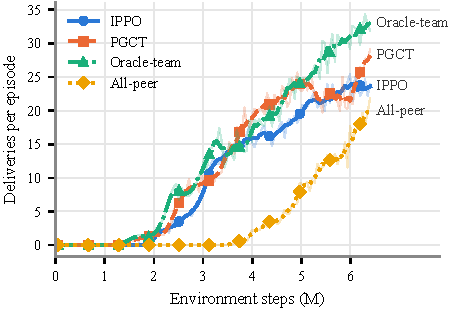
\includegraphics[width=\columnwidth]{figures/fig1_learning_curves.pdf}
\caption{Evaluation deliveries per episode on E1 (one seed\pilot). Thin: raw evaluations; thick: centred 5-point moving average.}
\label{fig:curves}
\end{figure}

\paragraph{Learning.} In this run \ours{} delivered more than IPPO on average (11.7 vs.\ 10.4 deliveries per episode, about
12\% more) and at the end (27.3 vs.\ 23.2, about 18\% more), and reached 20 deliveries per episode first (4.15M steps, against
4.66M for Oracle-team and 5.07M for IPPO; Table~\ref{tab:e1}, Figure~\ref{fig:curves}). All-peer started last. Per agent
(Appendix~\ref{app:e1}), IPPO trained one deliverer per team, \ours{} and Oracle-team trained a third agent, and All-peer trained all
four, late. These differences are within what one seed cannot resolve. The repeat run reproduced IPPO exactly up to 2.46M
steps but diverged for every transfer variant after 1.4--1.6M steps, presumably through nondeterministic operations on the
transfer path (Appendix~\ref{app:e1}). In the repeat, \ours{}'s onset came after IPPO's rather than before it, and All-peer's moved by
more than 2M steps. Measured from onset, the speed ranking depends on the threshold: $\Delta T_5$ was 0.77M for \ours{} and
0.82M for IPPO, $\Delta T_{10}$ 1.54M and 1.13M, and $\Delta T_{20}$ 2.41M and 3.02M. We therefore make no claim that \ours{}
learns faster than IPPO on E1. The late learning of a third agent under \ours{} and Oracle-team suggests that distilling a
competent agent's critic gives a signal to an agent that rarely receives reward itself; this needs an intervention that blocks
transfer to that agent \todo{intervention}.

\begin{figure*}[t]
\centering
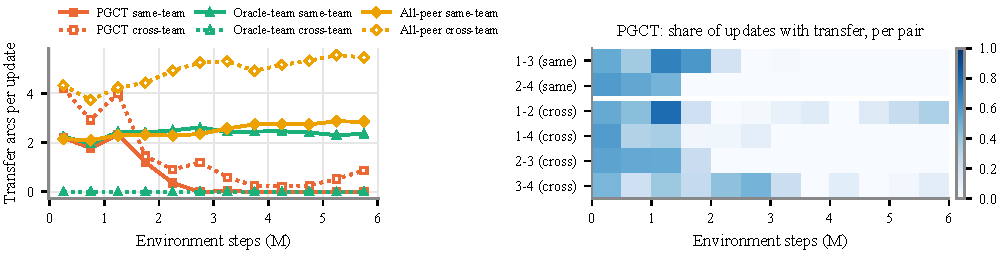
\includegraphics[width=\textwidth]{figures/fig3_critic_transfer.pdf}
\caption{Realised critic transfer on E1 (one seed\pilot). Left: directed transfer arcs per update within (solid) and across
(dotted) teams, 0.5M-step bins. Right: for \ours{}, share of updates in which each pair exchanged critic information.}
\label{fig:transfer}
\end{figure*}

\paragraph{Inference.} Proposition~\ref{prop:nonid} predicts that teams are not identifiable on E1, and the data agree. From
3M steps on, the probe divergence between teammates exceeded that between non-teammates at most checkpoints for all four
methods (Appendix~\ref{app:e1}), so the empirical margin was negative. After 4M steps, 95\% of \ours{}'s transfer arcs connected agents
of different teams (0.03 within-team vs.\ 0.63 cross-team arcs per update; Figure~\ref{fig:transfer}), mostly agents with the
same role: staying in the own half or fetching shelves from the other half. The gate also changed character during training.
Transfer occurred in 95\% of updates in the first 1M steps and in 12--19\% between 3M and 5M steps, because all pairwise
divergences grew as policies became more deterministic (teammates from 0.026 to 0.242 nats, non-teammates from 0.022 to 0.201)
and crossed the fixed $\tau$. Without a team signal, the fixed threshold acts as a schedule, close to All-peer early and close
to IPPO later, rather than as a teammate detector. Any gain on E1 therefore cannot come from transfer between teammates (H1).
It may come from selective transfer between behaviourally similar agents (H2) or from transferring less than All-peer (H3);
Random-gated will separate the two \todo{Random-gated on E1}. Consistent with H2, in frozen curriculum models of the E1 family,
blending a receiver's critic with a non-teammate's reduced its value error more than blending with a teammate's (same-team
AUROC 0.25--0.33).

\section{Offline Audit of Probe Statistics}
\label{sec:audit}
Before training on the main task we checked, on frozen models and without any training, whether the probe statistic carries a
team signal at all. Two model lineages are available on the E1 map. The curriculum lineage was trained in stages in which the
fraction of a team's shelves in its own half fell from 1.0 to 0.5 (stages 1--4), followed by continued training on E1. The
from-scratch lineage consists of the four E1 models of Section~\ref{sec:e1} at 6.4M steps. All models come from seed 1, and the
from-scratch models share initial weights, so they are independent training histories but not independent seeds. With four
agents there are two same-team and four cross-team pairs per model, so a single model's AUROC moves in steps of 1/8.
Table~\ref{tab:audit} summarises the results; 1 means teammates are always closer than non-teammates and 0.5 is chance.

\begin{table}[t]
\centering
\small
\resizebox{\columnwidth}{!}{%
\begin{tabular}{llcc}
\toprule
Statistic & Queries & Curriculum & From scratch \\
\midrule
Policy JS & v2 inference bank (48) & 0.12--0.62 & 0.38--0.50 \\
Policy JS & rule-based bank, team inputs neutral (32) & 0.67$^{a}$ & 0.25--0.62 \\
Policy JS & visited carrying windows, length 1 & 0.55--0.65 & 0.42--0.46 \\
Policy JS & visited carrying windows, length 12 & 0.47--0.62 & 0.42--0.46 \\
Reward model & designed probe states (240) & 0.38--0.62 & 0.25--0.50 \\
Reward model & visited carrying windows, length 1 & 0.97--1.00 & 0.71--0.79 \\
\quad on $Q_{\mathrm{diff}}$ / $Q_{\mathrm{same}}$ & & 1.00 / 0.95 & 0.79 / 0.58--0.67 \\
Event evidence$^{b}$ & own rollouts & 1.00 & -- \\
\bottomrule
\end{tabular}}
\caption{Same-team AUROC of probe statistics on frozen E1-map models (seed 1). Row 1: range over models; row 2: mean; window rows:
means over models, range over the two window-generating policies; 2--6 models per cell (Appendix~\ref{app:audit}). $Q_{\mathrm{diff}}$: queries whose actual reward differs between teams; $Q_{\mathrm{same}}$: the rest.
$^{a}$In-sample: the rule was chosen after inspecting these models. $^{b}$Observed pickups and deliveries of neighbours scored
against the observer's own goal; uses information that \ours{} does not exchange.}
\label{tab:audit}
\end{table}

\paragraph{Policy probes and shared space.} In the first curriculum stage, where each team works in its own half, the canonical
probe divergence separated the teams perfectly (AUROC 1.00), and the hard gate linked exactly the four within-team arcs. As
the stages mixed the teams' working areas, the AUROC fell to 0.62, 0.50 and 0.50, and the E1 models reached 0.38. In the
first stage team and zone coincide, so this shows that probes separate groups whose decisions on the probe states differ,
not that they find teams as such. Replacing the hard threshold by a sigmoid or softmax weighting did not help: with the
team signal of the later models the weight on teammates stayed around or below the chance level of 1/3 (0.08--0.35), whereas
where a signal existed the sigmoid put 0.97--1.00 of the weight on teammates. A soft rule changes the decision, not the
information.

\paragraph{Drift is as large as the team signal.} Propositions~\ref{prop:recovery} and \ref{prop:tracking} require drift that
is small relative to the margin. On E1, the divergence of an agent from itself between checkpoints 1M steps apart was
0.076--0.127 nats for \ours{}, while the team signal (cross-team minus same-team divergence) was between $-0.072$ and $+0.006$.
On the interrupted E1-F runs, self-divergence over 0.256M steps was 0.012--0.106 nats and the team signal between $-0.077$
and $+0.029$. The margin was mostly negative, and where it was positive it was smaller than the drift over intervals of this
length, so the conditions of Proposition~\ref{prop:recovery} were not met in any run we have.

\paragraph{Selecting or reweighting probes.} Weighting probes by how well they separated teams in other curriculum models
raised the AUROC on held-out curriculum models to 0.62--0.88, and the probes that worked across models were route-choice states
far from the goals, where a loaded agent turns towards one side. A bank built from this observation (branching corridor
cells, no goal in view, team-relative inputs neutral, far from the goal row) reached a mean of 0.67 on the curriculum models,
but the rule was derived from them. On the from-scratch lineage, which was not used to design it, the same bank gave
0.25--0.62, and neither the designed probes nor the weights carried over; the curriculum signal is more likely a route habit
inherited from the stages with team zones than a property of teams. Weighting probes by reward magnitude gave the same result
as uniform weights. On early E1-F checkpoints (0.5--1.5M steps), the probes that separated teams changed between checkpoints
(mean Spearman correlation of per-probe margins $+0.23$ between consecutive checkpoints and $-0.07$ across runs), and no probe
separated teams in all five runs.

\paragraph{Trajectories instead of single steps.} Feeding length-12 windows from visited states through the recurrent policy,
with the hidden state carried, did not improve on single-step probes in either lineage (Table~\ref{tab:audit}), whichever
policy generated the windows. The one exception, the last step of windows in which the goal was seen early and then left the
view (curriculum lineage, 0.45 to 0.72), rests on eight windows and we do not interpret it.

\paragraph{Reward probes.} We also trained, for each agent, a reward model $\hat r_i(o,a)$ on the agent's own experience and
compared agents by $|\hat r_i-\hat r_j|$ on shared queries. On the designed probe states the reward models failed even when they
were accurate (validation $R^2$ 0.92--0.94 for curriculum stages 3 and 4; AUROC 0.62 and 0.38). Only 5 of the 240 queries had
a reward that depended on the team, as Remark~\ref{rem:reward} predicts for E1. Queried instead on windows taken from visited
states in which an agent carries a requested shelf, the same kind of model separated teams in both lineages: 0.97--1.00 in the
curriculum lineage and 0.71--0.79 in the from-scratch lineage, where the policy probe on the same windows gave 0.42--0.46. The
result held when the windows were generated by a from-scratch policy instead of a curriculum policy, so it is not an artefact
of the window source. To see what the reward models pick up, we replayed each window, copied the environment state at every
step, and recomputed the acting agent's reward with its team label set to red and to blue. On visited carrying windows the
reward differed between teams for 51--79\% of queries, against 2\% on the designed states. On these queries each reward model
correlated with the actual reward of its own team (0.33--0.77) and not with that of the other team ($-0.03$ to $0.10$), and in
the from-scratch lineage team separation was higher on $Q_{\mathrm{diff}}$ (0.79) than on $Q_{\mathrm{same}}$ (0.58--0.67).
The signal therefore comes mainly from each agent having learned its own team's reward on states it actually visits. In the
curriculum lineage separation stayed high on $Q_{\mathrm{same}}$ (0.95), so differences in visited states contribute there as
well.

\paragraph{What the audit implies.} Policy-probe divergence, as used by \ours{}, was not a reliable teammate signal in any
setting where teams share space, and its drift was comparable to whatever signal there was. Reward probes on visited states are
the only statistic that kept a signal across lineages. The evidence is still thin: three from-scratch models with shared
initial weights, one map, and team differences that come mostly from small shaping terms (progress and pickup terms of
0.002--0.15 per step), which may vanish with sparse rewards. Using them in the gate would also require agents to share query windows,
which makes the choice of window-generating policy part of the method. Under team reward, the reward-correlation baseline is a
strong competitor, since teammates' task rewards coincide in time; on a curriculum model trained with individual reward it gave
AUROC 0.12, and on team-reward models it has not been measured. We keep the policy probe as the gate of \ours{} for the main
experiment and evaluate the reward probe alongside it offline \todo{decide after main-task checkpoints}.

\section{Goal-Separated Teams}
\label{sec:main}
\paragraph{Interrupted E1-F run.} IPPO, All-peer, Oracle-team, \ours{} and \ours{}-v2 were trained on E1-F with individual
rewards (seed 1).
The runs stopped at 1.67--1.70M steps when the host process was restarted; the last checkpoint is at 1.54M steps. Up to that
point no method delivered reliably (IPPO had one evaluation with 0.05 deliveries per episode), so the run says nothing about
learning. The gate was not selective: \ours{} with the canonical bank used 1.5--2.3 of 4 possible within-team arcs and
3.5--3.7 of 8 cross-team arcs per update (about 0.40 vs.\ 0.44 of the available arcs), \ours{}-v2 about 0.27 of each. Over the
whole run, 32.9\% of \ours{}'s arcs were within-team, against 36.2\% for Random-gated replayed on the same neighbour graphs. On
the v2 inference bank at 1.54M steps, the closest pairs were non-teammates whose action habits matched (0.045 and 0.036 nats),
while teammates were further apart (0.128 and 0.229). Since team-specific behaviour can only appear after agents learn to
deliver, these observations do not test the method.

\paragraph{Main task.} Table~\ref{tab:main} lists what will be reported. \todo{Fill after the pilot and main runs on B (or A/C): (1) Oracle-team vs.\ Random-gated and All-peer;
(2) within- vs.\ cross-team compatibility; (3) within-team arc share against Random-gated, precision/recall, AUROC, $\Delta$
and $\rho$ for \ours{} and \ours{}-v2, and the reward-correlation baseline; (4) learning curves over seeds.}

\begin{table}[t]
\centering
\small
\resizebox{\columnwidth}{!}{%
\begin{tabular}{lcccccc}
\toprule
Method & Onset & Mean & Final & Within-team arcs & Recall & AUROC \\
\midrule
IPPO & \tbd & \tbd & \tbd & -- & -- & \tbd \\
All-peer & \tbd & \tbd & \tbd & \tbd & \tbd & -- \\
Random-gated & \tbd & \tbd & \tbd & \tbd & \tbd & -- \\
\ours{} & \tbd & \tbd & \tbd & \tbd & \tbd & \tbd \\
\ours{}-v2 & \tbd & \tbd & \tbd & \tbd & \tbd & \tbd \\
Oracle-team & \tbd & \tbd & \tbd & 1 & \tbd & -- \\
\midrule
Reward correlation & -- & -- & -- & -- & -- & \tbd \\
\bottomrule
\end{tabular}}
\caption{Main task (B unless the pilot selects A or C), mean over \tbd{} seeds. Within-team arcs: share of realised transfer
arcs that connect teammates. Recall: share of available within-team arcs that were used. AUROC of the probe divergence on
checkpoints; reward correlation is an identification reference only. \todo{fill when the runs finish}}
\label{tab:main}
\end{table}

\section{Discussion and Limitations}
\paragraph{What the analysis gives.} Propositions~\ref{prop:recovery}--\ref{prop:bias} turn the informal chain ``similar
behaviour, hence same team, hence useful critic'' into conditions that can be checked: a positive margin, drift that is small
relative to it, and compatible values among teammates. Propositions~\ref{prop:counter} and \ref{prop:nonid} show that the
chain can break, and E1 is an instance of the second break. The audit adds that in our models the drift condition failed as well,
including early checkpoints of the goal-separated task, where the symmetry argument does not apply. We give no convergence result for the coupled learning dynamics.

\paragraph{A gate without a signal is a schedule.} When the probe divergence carries no team information, \ours{} does not
reduce to independent learning. Because all divergences start small and grow with training, a fixed $\tau$ first admits almost
every neighbour and later almost none. This explains why the E1 gate behaved like All-peer early and like IPPO late, and it is
why Random-gated, matched to the realised number of arcs at every update, is the control that matters. A threshold set relative
to each agent's own drift, or to the distribution of divergences among its neighbours, would remove the dependence on the
learning stage but would not create information.

\paragraph{Team discovery remains the target.} One could redefine the goal as finding useful donors regardless of team (Q2).
We keep teammate inference (Q1) as the aim and treat compatibility as something to verify, because team relations are what a
designer usually wants respected, and because Q2 can be estimated by Oracle-team and Random-gated without changing the method.
If the main task shows that teammates are not better donors, that is a result about the premise and will be reported as such.

\paragraph{Assumptions and scope.} \ours{} needs a shared probe bank that satisfies Assumption~\ref{as:comparability}. Our banks
are built by fixed rules from the map, but the audit shows that results depend on the query set more than on the rule that
produced it, and that query sets tuned on one lineage do not transfer. Agents could exchange team identifiers if they had a
common vocabulary; teammate inference is relevant when objectives are private or labels are not shared. All results so far come
from one environment family, four agents, two teams and one seed, and the transfer variants are not deterministic even at a
fixed seed. Team reward, used in the main task, restricts the claim to cooperative latent teams.

\section{Conclusion}
\ours{} infers local teammates from responses to a shared probe bank and distils their critics. We stated the conditions under
which this is justified (separation, bounded drift, compatible values) and when they fail, including a non-identifiability
result for teams whose decision problems coincide. On a team-symmetric task the gate did not find teams, as predicted, and the
single-seed performance difference to IPPO was within run-to-run variation. Offline, policy-probe divergence did not separate
teams once they shared space, while reward models queried on visited states did, mostly through each agent's own-team reward.
Whether \ours{} recovers teams and helps when the conditions can hold is the question for the goal-separated main task.

\ifdefined\ijcaistyle
  \bibliographystyle{named}
\else
  \bibliographystyle{plainnat}
\fi
\bibliography{references_v04}

\clearpage
\appendix
\onecolumn

\section{Proofs}
\label{app:proofs}

\textbf{Proposition~\ref{prop:properties}.}
(a) For $m=\frac{p+q}{2}$, $\KL(p\Vert m)=\sum_a p(a)\ln\frac{2p(a)}{p(a)+q(a)}\le\sum_a p(a)\ln 2=\ln 2$, and similarly for $q$; hence
$0\le\JS\le\ln2$. Symmetry is immediate. $\JS(p,q)=0$ iff $\KL(p\Vert m)=\KL(q\Vert m)=0$ iff $p=m=q$. Averaging over probes preserves
all three statements, with equality to zero iff every term is zero.
(b) $\JS(p,q)=\sum_a q(a)\,\phi\!\big(p(a)/q(a)\big)$ with $\phi(t)=\frac{t}{2}\ln\frac{2t}{1+t}+\frac12\ln\frac{2}{1+t}$, which is convex
with $\phi(1)=0$; $\JS$ is therefore an $f$-divergence, and $f$-divergences are jointly convex in their two arguments (perspective of a
convex function). A sum of jointly convex functions of disjoint coordinates is jointly convex.
(c) $\sqrt{\JS}$ is a metric on $\Delta(\mathcal{A})$ \cite{endres2003metric}. For $x_m=\sqrt{\JS(p_i^m,p_k^m)}$,
$y_m=\sqrt{\JS(p_i^m,p_j^m)}$, $w_m=\sqrt{\JS(p_j^m,p_k^m)}$ we have $x_m\le y_m+w_m$, and by Minkowski's inequality
$\big(\frac1M\sum_m x_m^2\big)^{1/2}\le\big(\frac1M\sum_m y_m^2\big)^{1/2}+\big(\frac1M\sum_m w_m^2\big)^{1/2}$, i.e.\
$d_{ik}\le d_{ij}+d_{jk}$. Symmetry and $d_{ii}=0$ follow from (a). It is a pseudometric because policies that agree on $\mathcal{Q}$ have
$d=0$.

\textbf{Proposition~\ref{prop:recovery}.} If $z_i=z_j$, then $\bar D_{ij}\le D_{ij}+\epsilon\le\delta_{\mathrm{in}}+\epsilon<\tau$, so
$j\in\hat{\mathcal{T}}_i$. If $z_i\ne z_j$, then $\bar D_{ij}\ge D_{ij}-\epsilon\ge\delta_{\mathrm{out}}-\epsilon>\tau$, so
$j\notin\hat{\mathcal{T}}_i$. The interval for $\tau$ is non-empty iff $2\epsilon<\Delta$. Symmetry follows because the conditions do not
depend on the order of $i$ and $j$.

\textbf{Lemma~\ref{lem:drift}.} By joint convexity of $\KL$, $\KL(p\Vert\frac{p+p'}{2})\le\frac12\KL(p\Vert p)+\frac12\KL(p\Vert p')=\frac12\KL(p\Vert p')$,
and likewise $\KL(p'\Vert\frac{p+p'}{2})\le\frac12\KL(p'\Vert p)$. Hence $\JS(p,p')\le\frac14(\KL(p\Vert p')+\KL(p'\Vert p))\le\kappa/4$. By the
triangle inequality for $\sqrt{\JS}$ on each probe,
$|\sqrt{\JS(p_i'^m,p_j'^m)}-\sqrt{\JS(p_i^m,p_j^m)}|\le\sqrt{\JS(p_i^m,p_i'^m)}+\sqrt{\JS(p_j^m,p_j'^m)}\le\sqrt{\kappa}$. Minkowski's
inequality over probes gives $|d'_{ij}-d_{ij}|\le\sqrt{\kappa}$, and $|D'-D|=|d'-d|(d'+d)\le\sqrt{\kappa}\cdot2\sqrt{\ln 2}$ by
Proposition~\ref{prop:properties}(a).

\textbf{Proposition~\ref{prop:tracking}.} Let $e_n=\bar D(n)-D(n)$. Then $e_n=(1-\beta)\bar D(n-1)+\beta D(n)-D(n)=(1-\beta)e_{n-1}+(1-\beta)(D(n-1)-D(n))$,
so $|e_n|\le(1-\beta)|e_{n-1}|+(1-\beta)\rho$. With $e_1=0$ (initialisation with the first measurement),
$|e_n|\le(1-\beta)\rho\sum_{k\ge0}(1-\beta)^k=\frac{1-\beta}{\beta}\rho$.

\textbf{Proposition~\ref{prop:bias}.} $f''(v)=2c+2\lambda\sum_j\alpha_{ij}=2(c+\lambda)$, so $f$ is $2(c+\lambda)$-strongly convex and has the
unique stationary point $v^\star$ given. Then $v^\star-y=\frac{\lambda}{c+\lambda}\sum_j\alpha_{ij}(v_j-y)$, and the triangle inequality with the
stated bounds on $|v_j-y|$ gives the result.

\textbf{Proposition~\ref{prop:counter}.} Take a single state, a single action and $\mathcal{Q}=\{q\}$ with both agents' policies the point mass on that
action, so $D_{ij}=0$. Let $r_i\equiv0$ and $r_j\equiv1$; then $V_i=0$ and $V_j=\sum_t\gamma^t=1/(1-\gamma)$.

\textbf{Proposition~\ref{prop:nonid}.} With the other agents fixed, the expected discounted return of a memoryless map $\mu$ for agent $i$ is a
functional of the law of the observation--reward sequence that $i$ experiences under $\mu$. If these laws coincide for agents $i$ and $j$ of
different teams for every $\mu$, then every $\mu$ has the same return for both, so the sets of optimal memoryless maps coincide. If the optimal
map $\mu^\star$ is unique, every objective-optimal policy equals $\mu^\star$ on every observation, including every probe, so $p_i^m=p_j^m$ and
$D_{ij}=0$ for all pairs. Then $\delta_{\mathrm{in}}=\delta_{\mathrm{out}}=0$ and $\Delta=0$, and no $\tau$ satisfies
$\delta_{\mathrm{in}}<\tau\le\delta_{\mathrm{out}}$.

\section{Hyper-parameters}
\label{app:hyper}
\begin{table}[h]
\centering
\small
\begin{tabular}{ll}
\toprule
Setting & Value \\
\midrule
Map / agents / teams & 11$\times$10 E1 / 4 / 2 \\
Reward & individual \\
Home-zone shelf ratio & 0.5 \\
Requests per team & 2 \\
Sensor / communication range & 5 / 5 \\
Learning rate & 0.0002 \\
Entropy coef. & 0.05 \\
$\gamma$ / GAE $\lambda$ & 0.99 / 0.95 \\
Rollout / BPTT length & 1024 / 64 \\
PPO epochs / minibatches / clip & 4 / 8 / 0.2 \\
Hidden (MLP / GRU) & 128 / 128 \\
Peer-loss coef. $\lambda_{peer}$ & 0.01 \\
Gate: JS threshold / EMA $\beta$ / warm-up & 0.12 / 0.35 / 100 upd. \\
Canonical probes & 48 (fixed, zero hidden, length 1) \\
Evaluation & every 50 updates, 20$\times$500 steps, deterministic \\
\bottomrule
\end{tabular}

\caption{Settings of the from-scratch E1 comparison (identical for all methods except the donor set). The main task B differs in
the number of agents (6), requests per team (3), communication range (3), team reward and goal positions.}
\end{table}

\section{Realised transfer per window}
\begin{table}[h]
\centering
\small
\begin{tabular}{llccc}
\toprule
Method & Window & Updates w/ transfer & Same-team arcs/upd. & Cross-team arcs/upd. \\
\midrule
PGCT & 0--2.0M & 91\% & 1.86 & 3.09 \\
 & 2--4.0M & 37\% & 0.10 & 0.73 \\
 & 4--6.4M & 29\% & 0.03 & 0.63 \\
\addlinespace
Oracle-team & 0--2.0M & 82\% & 2.26 & 0.00 \\
 & 2--4.0M & 86\% & 2.50 & 0.00 \\
 & 4--6.4M & 85\% & 2.39 & 0.00 \\
\addlinespace
All-peer & 0--2.0M & 99\% & 2.22 & 4.18 \\
 & 2--4.0M & 100\% & 2.49 & 5.10 \\
 & 4--6.4M & 100\% & 2.79 & 5.37 \\
\bottomrule
\end{tabular}

\caption{Realised transfer on E1 per training window (one seed). Arcs are directed receiver--donor links.}
\end{table}

\section{Additional E1 results}
\label{app:e1}
\begin{figure}[h]
\centering
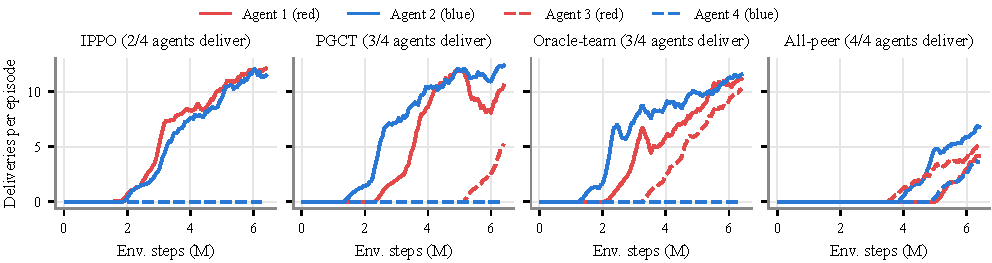
\includegraphics[width=\textwidth]{figures/fig2_per_agent_deliveries.pdf}
\caption{Deliveries per episode of each agent on E1 (5-point moving average; one seed). Red: team red (agents 1, 3); blue: team blue
(agents 2, 4); solid: agents 1--2; dashed: agents 3--4.}
\end{figure}
\begin{figure}[h]
\centering
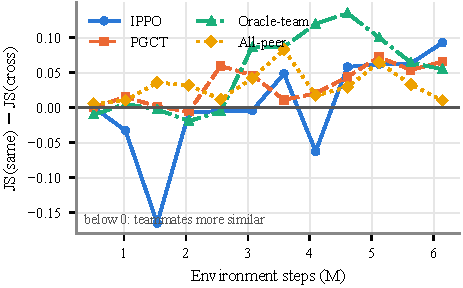
\includegraphics[width=0.6\textwidth]{figures/fig4_probe_js_gap.pdf}
\caption{Probe divergence between teammates minus that between non-teammates on E1 checkpoints (one seed). Above zero: teammates differ
more, i.e.\ the empirical margin is negative.}
\end{figure}
\begin{figure}[h]
\centering
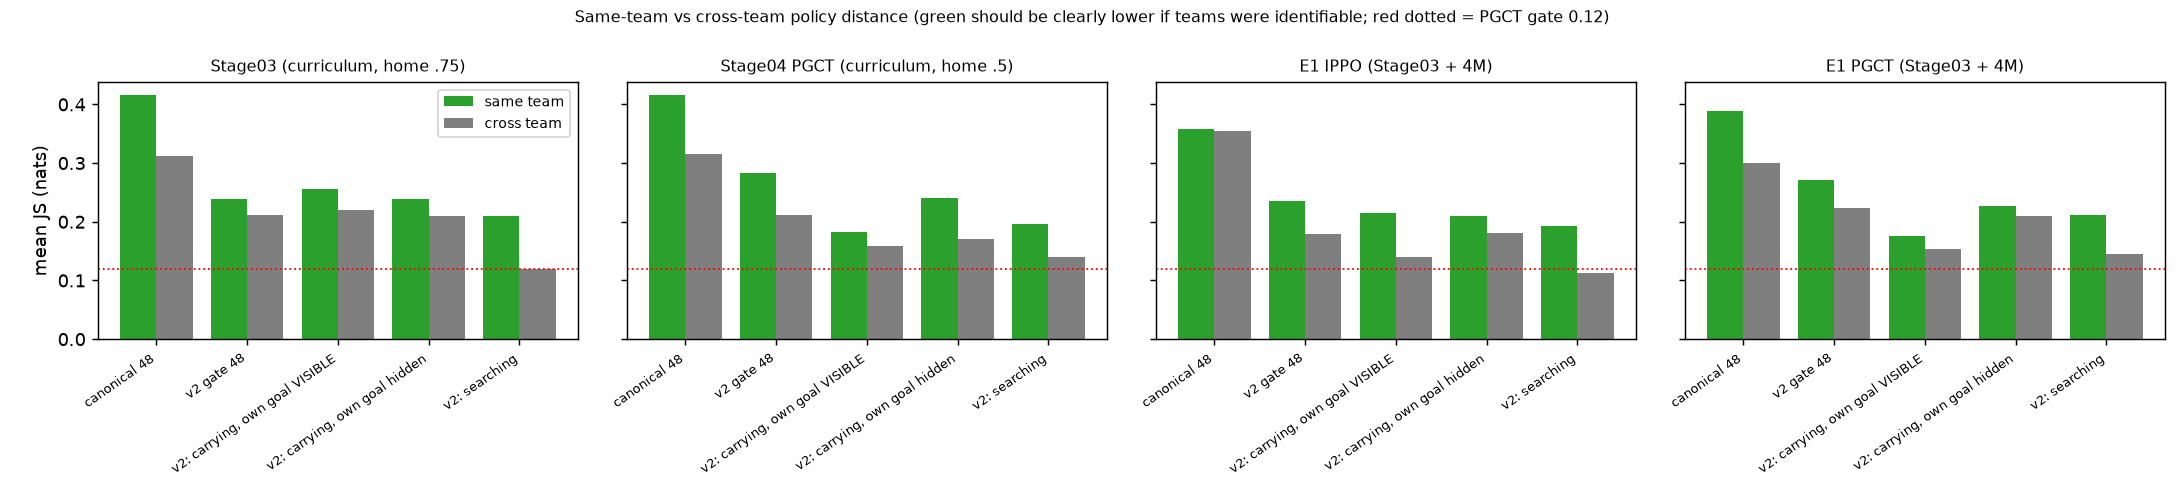
\includegraphics[width=\textwidth]{figures/frozen_probe_same_vs_cross.png}
\caption{Mean probe divergence between teammates (green) and non-teammates (grey) for four frozen E1 models of the curriculum lineage and
five probe subsets, including the v2 inference bank. Teammates are less similar in all 20 combinations. Red dotted line: $\tau=0.12$.}
\end{figure}
\begin{figure}[h]
\centering
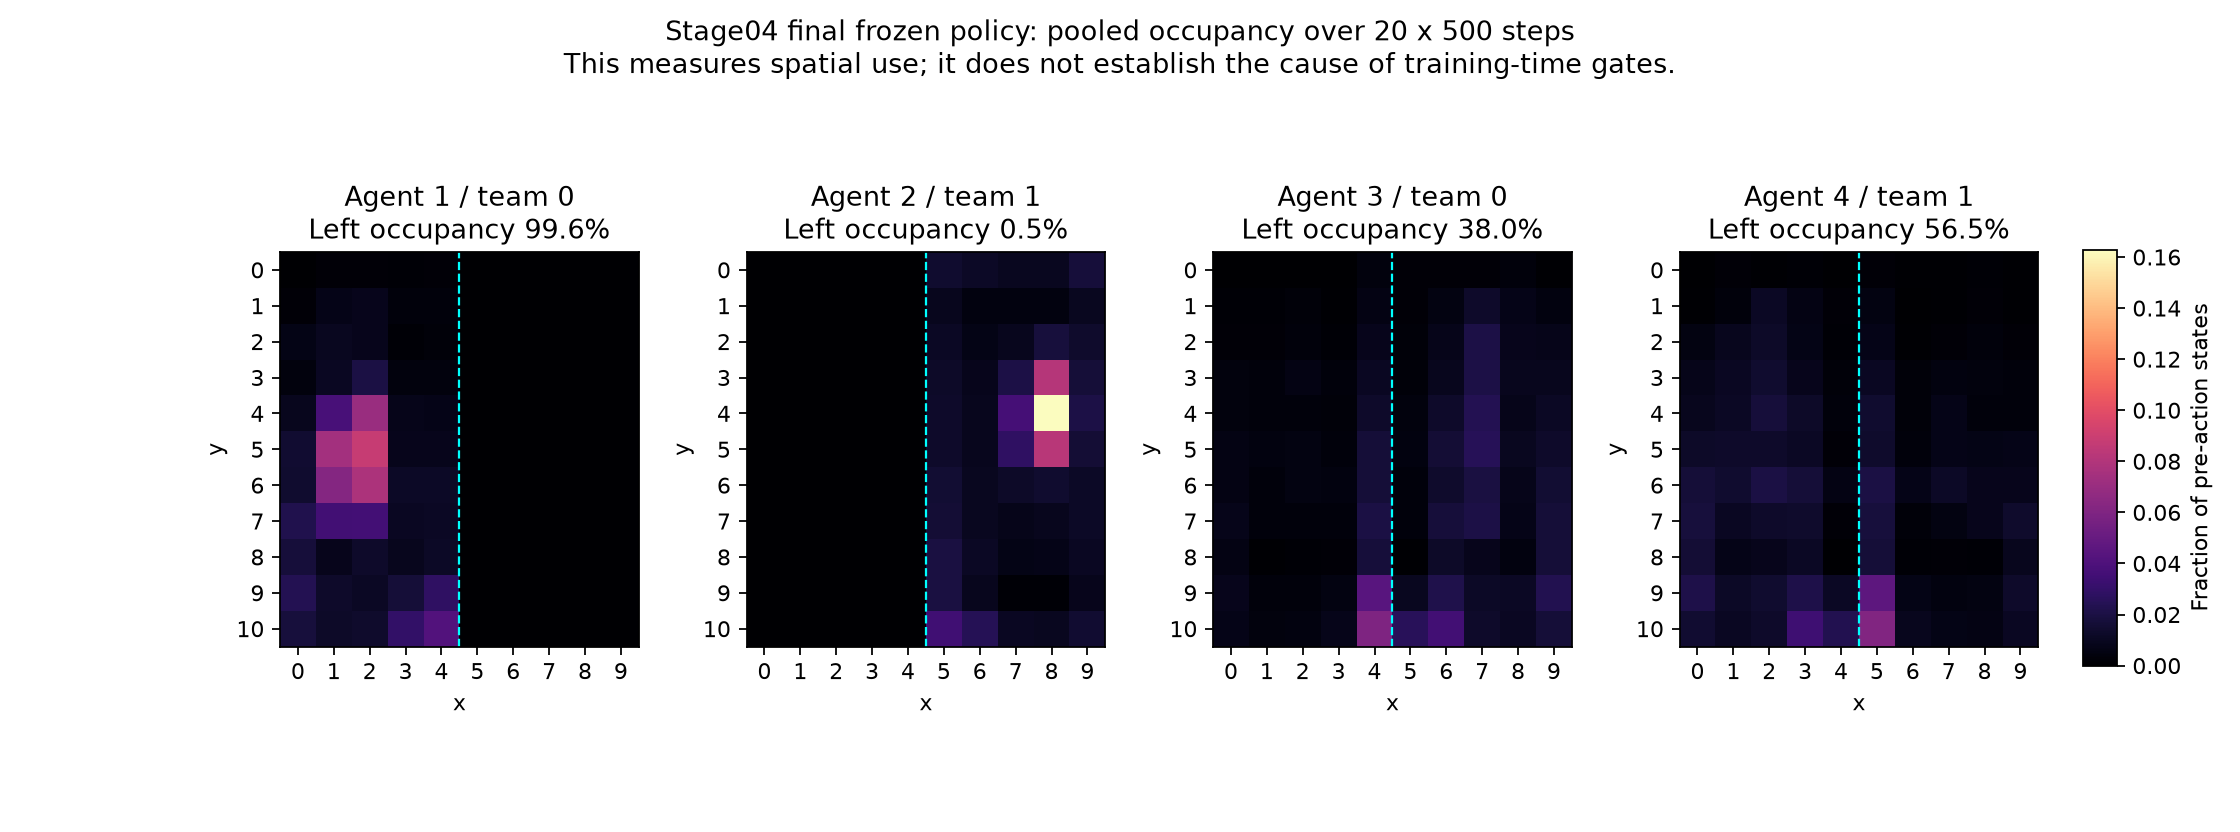
\includegraphics[width=\textwidth]{figures/stage04_occupancy.png}
\caption{Cell occupancy of a frozen curriculum model (50\% of shelves in the other team's half). Agents 1 and 2 stay in their team's half;
agents 3 and 4 fetch shelves from the other half and are the pair the gate linked most often.}
\end{figure}
\begin{figure}[h]
\centering
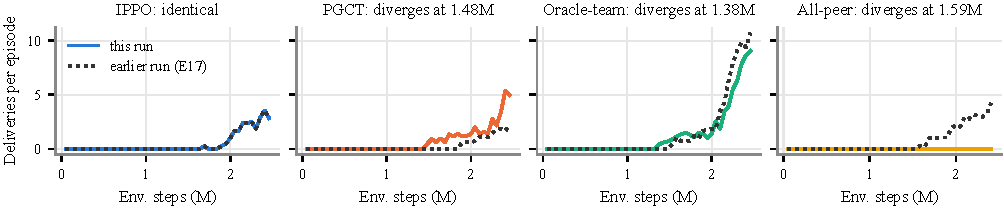
\includegraphics[width=\textwidth]{figures/figA1_reproducibility.pdf}
\caption{Same seed and initial weights, two runs (solid: reported; dotted: earlier interrupted run). IPPO is reproduced exactly; the sharing
variants diverge after 1.4--1.6M steps.}
\end{figure}

\section{Audit details}
\label{app:audit}
All audit computations use frozen weights (hashes checked before and after) and no agent training; reward models and rollouts are
the only things trained or generated.

\textbf{Models.} Curriculum lineage: stage models 1--4 (fraction of a team's shelves in its own half 1.0, 0.875, 0.75, 0.5) and two models
continued on E1 (IPPO and \ours{}); some analyses also include two models on a $16\times16$ map. From-scratch lineage: IPPO, \ours{},
Oracle-team and All-peer of Section~\ref{sec:e1} at 6.4M steps. When a model generated the query windows, it was excluded from scoring, so
the from-scratch cells of the window rows in Table~\ref{tab:audit} use three models.

\textbf{Policy probes.} Same rule as the gate: zero hidden state, unmasked, natural-log JS averaged over probes. The rule-based bank uses
corridor cells with at least three free directions, no goal in view, team-relative inputs set to a neutral value, and a band far from the
goal row (32 states); the band was chosen after inspecting curriculum probes. Visited windows: 60 episodes of 500 steps of a generating
policy (curriculum stage 4 or from-scratch All-peer), windows of 12 steps drawn evenly over the generating agents without team labels;
``carrying'' windows have the agent carrying a requested shelf.

\textbf{Reward probes.} One MLP per agent on (observation, one-hot action), trained on 20 episodes of 500 steps of the model's own
stochastic policy, three initialisation seeds; distance $|\hat r_i-\hat r_j|$ averaged over queries. Counterfactual split: every source
episode was replayed from its reset seed and recorded joint actions (all 3{,}804 checked rewards matched the record); at each step the
environment was copied and the acting agent's team was set to red and to blue before executing the same joint action. Mean
$|r_{\mathrm{red}}-r_{\mathrm{blue}}|$ on $Q_{\mathrm{diff}}$ was 0.002--0.051, mostly shaping terms.

\textbf{Drift.} Self-divergence is $D$ between an agent's responses at two checkpoints, computed on the bank used by its gate. It is not the
per-measurement $\rho$ of Proposition~\ref{prop:tracking}, which refers to changes between measurements five updates apart; we report it
because it can be computed from saved checkpoints \todo{per-measurement $\rho$ from communication logs}.

\end{document}
